\chapter{Experiments}
\label{chap:experiments}
In this chapter, we describe a set of experiments we ran to quantitatively and qualitatively measure the effect of incorporating the log embeddings introduced into normal behavior models
when applied to both \emph{healthy} and \emph{faulty} turbines. For a normal behavior model monitoring a component of a turbine, we considered this turbine \emph{faulty} if 
a failure was reported, in the failures dataset, related to this specific component of this turbine. It is considered \emph{healthy} if no failures, relating to this turbine's component,
were reported.\\
To compare different models in an identical setup, we use the following metrics:
\begin{bulletList}
    \item \textbf{Root Mean Squared Error ($RMSE$)}: It is a commonly used metric to evaluate the performance of a predictive model or an estimator.
    The $RMSE$ is calculated as the square root of the mean of the squared differences between the predicted ($y_{predicted}$) and actual values ($y_{actual}$), or as follows:
    \begin{equation}
        RMSE = \sqrt{\frac{1}{n} * \sum_{i}^{n} (y_{predicted}^i - y_{actual}^i)^2}
    \end{equation}
    where $n$ is the number of data points in a dataset. The RMSE is expressed in the same units as the original data. 
    As a rule of thumb: The lower the RMSE, the better the model fits the data.
    \item \textbf{Numbers of anomalies and alarms detected during a given period}: We use these numbers to measure the capability of a model to detect/predict a failure. 
    The number of anomalies detected reflects the total number of anomalous data points, whereas the number of alarms detected counts only the number of operation days of a turbine 
    where the system notified the operator of a potential failure by sending an alarm (if the number of anomalies detected in a day exceeds a certain threshold, 
    as explained in \ref{subsub:anvsal}). When compared to another model, we consider a model more \emph{capable} of predicting failures if it 
    detects more anomalies and/or sends more alarms during the time of abnormal operation of a faulty turbine given that it reported no anomalies or alarms during the normal operation 
    of the same turbine. In other words, we compare these metrics between models when applied to the test data of a faulty turbine, assuming that the data used to train these models 
    was collected from the turbine in a period when it was operating in a healthy state; hence no anomalies should be detected in this period.
    \item \textbf{Timestamps of the first anomaly detected and alarm sent}: Used to compare the capability of different models to early-detect failures, when applied to a faulty turbine. The earlier
    the first anomaly is detected or the first alarm is sent the better.
\end{bulletList}
All the condition monitoring normal behavior models used in our experiments were trained to monitor the generator bearings of a turbine (i.e., having the average temperature in the generator bearings 
as a target), whereas the power curve normal behavior models monitor the average power production of a turbine according to the grid (in kW). The input features used are listed in \ref{sub:featselect}.

%Experiment I
\section{Benchmark NBM architecture}
\label{exp:I}

In the early stages of this work, we trained linear regression models due to their lightweight and low computational power needed. Knowing that they are incapable of capturing non-linear
relationships in the data, we assumed that the linear regression models would be outperformed by feed-forward neural networks when it comes down to fitting the 
signals data of a healthy turbine. To test this hypothesis and select a specific architecture to be used as a benchmark NBM model in other experiments, we did this simple experiment 
to compare the $RMSE$ scores of both models.\\
This experiment was conducted on a healthy turbine (Turbine 01). Both models were trained on signals data collected between 01/09/2016 and 30/08/2017 and tested on data collected between
01/09/2017 and 31/12/2017.\\
As shown in Table \ref{tab:Experiment I results}, the feed-forward network outperformed the linear regression model---as expected---and was used as a baseline in all the other experiments.
\begin{table}[H]
        \centering
    \begin{tabular}{|c|c|c|}
    \hline
         \textbf{Metric} & \textbf{Linear regression} & \textbf{Feed-forward network}\\
         \hline
         Training RMSE & 5.29 & 4.86\\
         \hline
         Testing RMSE & 5.80 & 5.78 \\
    \hline
    \end{tabular}
    \caption{Experiment I results: RMSEs measured and used to compare between the benchmark models}
        \label{tab:Experiment I results}
\end{table}

%Experiment II

\section{Effect of incorporating log embeddings into NBM for condition monitoring when applied to a healthy turbine (T01)}
\subsection{Setup}
This experiment aims to quantitatively and qualitatively measure 
the effect of incorporating SCADA-log-based embeddings into the baseline normal behavior model when applied to a healthy turbine.
(see method \ref{sub:dk_method} and \ref{subsub:Loglizer})\\
We ran this experiment three times: one time using the baseline normal behavior model (i.e., using only SCADA signals as input features), 
repeated once after adding the log embeddings generated based on domain knowledge as input features (denoted as \emph{Model-DK}) and 
another time after incorporating LogPAI-generated log embeddings (denoted as \emph{Model-PAI}).
The models were trained on data collected between 01/09/2016 and 30/08/2017 and tested on data collected between
01/09/2017 and 31/12/2017.\\
As shown in Table \ref{tab:expII:domain-knowledge-feats}, all log embeddings generated based on domain knowledge highly correlate with the target feature 
and were hence used as input features in \emph{Model-DK} in addition to the selected SCADA signals.
As for the log embeddings generated using LogPAI, only a few features were found to relatively highly correlate (correlation factor greater than 0.3 or less than -0.3) 
with the target feature (see Table \ref{tab:expII:logpai-feats}) and were selected, in addition to the selected SCADA signals, as input features in \emph{Model-PAI}.
\begin{table}[H]
    \parbox{.45\linewidth}{
    \centering
    \begin{tabular}{|c|c|}
        \hline
        Feature & Correlation\\
        \hline
        \multicolumn{1}{|m{0.25\textwidth}|}{Generator external ventilator} & 0.713057\\
        \hline
        \multicolumn{1}{|m{0.25\textwidth}|}{Generator internal ventilator} & 0.730726\\
        \hline
        \multicolumn{1}{|m{0.25\textwidth}|}{High-voltage transformer ventilator} & 0.513700\\
        \hline
        \multicolumn{1}{|m{0.25\textwidth}|}{Nacelle ventilator} & 0.514112\\
        \hline
    \end{tabular}
    \caption{Measures of Kendall's correlation between the domain knowledge-based log embeddings and the target feature in Turbine 01}
    \label{tab:expII:domain-knowledge-feats}
    }
    \hfill
    \parbox{.45\linewidth}{
    \centering
    \begin{tabular}{|c|c|}
        \hline
        Feature & Correlation\\
        \hline
        \multicolumn{1}{|m{0.25\textwidth}|}{\hl{LogPAI Feature 1}} & \hl{-0.335313}\\
        \hline
        \multicolumn{1}{|m{0.25\textwidth}|}{\hl{LogPAI Feature 2}} & \hl{-0.320031}\\
        \hline
        \multicolumn{1}{|m{0.25\textwidth}|}{LogPAI Feature 3} & 0.015902\\
        \hline
        \multicolumn{1}{|m{0.25\textwidth}|}{LogPAI Feature 4} & -0.220749\\
        \hline
        \multicolumn{1}{|m{0.25\textwidth}|}{LogPAI Feature 5} & 0.083943\\
        \hline
        \multicolumn{1}{|m{0.25\textwidth}|}{\hl{LogPAI Feature 6}} & \hl{-0.303429}\\
        \hline
        \multicolumn{1}{|m{0.25\textwidth}|}{LogPAI Feature 7} & 0.191848\\
        \hline
        \multicolumn{1}{|m{0.25\textwidth}|}{LogPAI Feature 8} & -0.045460\\
        \hline
        \multicolumn{1}{|m{0.25\textwidth}|}{LogPAI Feature 9} & -0.077507\\
        \hline
        \multicolumn{1}{|m{0.25\textwidth}|}{LogPAI Feature 10} & -0.157537\\
        \hline
        \multicolumn{1}{|m{0.25\textwidth}|}{LogPAI Feature 11} & -0.102636\\
        \hline
        \multicolumn{1}{|m{0.25\textwidth}|}{LogPAI Feature 12} & 0.018344\\
        \hline
        \multicolumn{1}{|m{0.25\textwidth}|}{LogPAI Feature 13} & 0.244219\\
        \hline
        \multicolumn{1}{|m{0.25\textwidth}|}{LogPAI Feature 14} & -0.129601\\
        \hline
        \multicolumn{1}{|m{0.25\textwidth}|}{\hl{LogPAI Feature 15}} & \hl{0.361669}\\
        \hline
        \multicolumn{1}{|m{0.25\textwidth}|}{LogPAI Feature 16} & -0.010470\\
        \hline
    \end{tabular}
    \caption{Measures of Kendall's correlation between the log embeddings generated based on the event IDs using the LogPAI framework and the target feature in Turbine 01. Selected features are highlighted.}
    \label{tab:expII:logpai-feats}
    }
    \end{table}

At this stage, the main goal is to test whether those highly-correlating features would improve the baseline model, or, 
they provide redundant information that could be indirectly deduced from the signal features.

\subsection{Results}
\subsubsection{Performance}
As reported in Table \ref{tab:Experiment II results}, the incorporated log embeddings, both in \emph{Model-DK} and \emph{Model-PAI}, improved the RMSE scores of the models. 
This shows that those features provided additional information to the model that wasn't available in the selected SCADA signals, which shows that our proposed methods 
were indeed capable of retrieving valuable information from the SCADA logs.

\begin{table}[H]
    \centering
\begin{tabular}{|c|c|c|c|}
\hline
     \textbf{Metric} & \textbf{\emph{Baseline}} & \textbf{\emph{Model-DK}} & \textbf{\emph{Model-PAI}}\\
     \hline
     Training RMSE & 4.864 & 4.087 & 4.617\\
     \hline
     Testing RMSE & 5.784 & 5.195 & 5.607\\
\hline
\end{tabular}
\caption{Experiment results: RMSEs measured and used to compare between the \emph{Baseline} model, \emph{Model-DK} and \emph{Model-PAI} when applied to Turbine 01}
    \label{tab:Experiment II results}
\end{table}

\subsubsection{Anomaly detection}
Applying the models to the testing dataset, 12, 15 and 8 data points were labeled anomalous by the \emph{Baseline} model,
\emph{Model-DK} and \emph{Model-PAI}, respectively. Whether to consider these data points as false positives or not is 
arguable. One could consider them as false positives based on the premise that the turbine was operating in a healthy state.
In this case, \emph{Model-PAI} would be ranked highest in terms of anomaly detection. However, these data points could indeed
be anomalous and be signaling a fault that might happen in the future. Here, \emph{Model-DK} would show a higher sensitivity 
to anomalous data points. \\
Given that the dataset provided doesn't include data from the following years (2018+), 
we weren't able to test the different possibilities and will leave the interpretation open to the reader.\\

No alarms were reported in all three models. This result shows that none of the anomalies detected was considered 
critical enough for the operator to be notified, which aligns with the assumption that the turbine is healthy.




%Experiment III

\section{Effect of incorporating log embeddings into NBM for condition monitoring when applied to a faulty turbine (T09)}
\subsection{Setup}
This experiment aims to quantitatively and qualitatively measure 
the effect of incorporating SCADA-log-based embeddings into the baseline normal behavior model when applied to a faulty turbine 
(see method \ref{sub:dk_method}, \ref{subsub:vis_warnings} and \ref{subsub:Loglizer}).\\
For this turbine (T09), several failures relating to the generator bearings were reported starting on 07/06/2016 and ending on 17/10/2016
by replacing the generator bearings (see Table \ref{tab:failures}). In this case, not only do we want to measure the performance of our models fitting the data 
during the presumably healthy (training) period, but also we want to test their capability of detecting the recorded failures early and notifying the operator 
in cases of major anomalies in the operation of the turbine's component.\\
We ran this experiment three times: one time using the baseline normal behavior model (i.e., using only SCADA signals as input features), 
repeated once after adding the log embeddings generated based on domain knowledge as input features (denoted as \emph{Model-DK}) and 
another time after incorporating LogPAI-generated log embeddings (denoted as \emph{Model-PAI}).
The models were trained on data collected between 01/01/2016 and 15/02/2016 and tested on data collected between
16/02/2016 and 18/10/2016. Due to the limits of the dataset at hand, only two and a half months of data could be used to train the models since, 
according to our analysis, this is the period where the turbine was assumably still operating in healthy conditions.
Due to the shortage in the training dataset, some features in the testing dataset were found to be out-of-distribution (see Fig. \ref{fig:Boxplot_T09}). 
This fact made the interpretation of the results a bit more challenging, it, however, helped test the robustness of the 
different models' architectures.

\begin{figure}[H]
    \begin{center}
      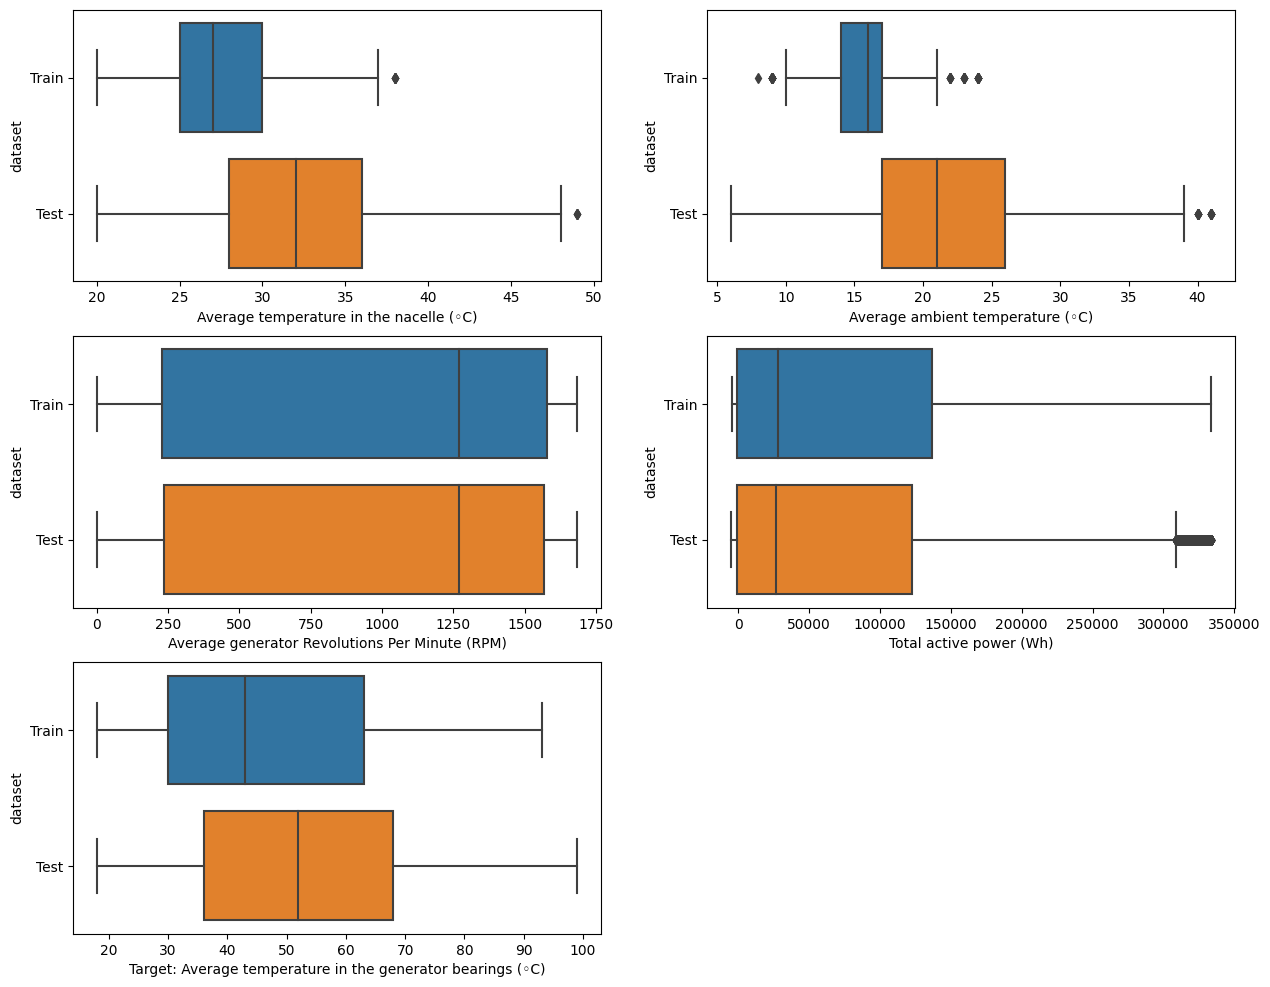
\includegraphics[scale=0.43]{Experiments/Boxplot_T09.png}
    \end{center}
    \caption{Boxplots showing the distribution of signals collected from Turbine 09 sensors used to train and test the models}
    \label{fig:Boxplot_T09}
  \end{figure}

As shown in Table \ref{tab:expIII:domain-knowledge-feats}, all log embeddings generated based on domain knowledge highly correlate with the target feature 
and were hence used as input features in \emph{Model-DK} in addition to the selected SCADA signals.
As for the log embeddings generated using LogPAI, only a few features were found to relatively highly correlate (correlation factor greater than 0.3 or less than -0.3) 
with the target feature (see Table \ref{tab:expIII:logpai-feats}) and were selected, in addition to the selected SCADA signals, as input features in \emph{Model-PAI}.
\begin{table}[H]
    \parbox{.45\linewidth}{
    \centering
    \begin{tabular}{|c|c|}
        \hline
        Feature & Correlation\\
        \hline
        \multicolumn{1}{|m{0.25\textwidth}|}{Generator external ventilator} & 0.505995\\
        \hline
        \multicolumn{1}{|m{0.25\textwidth}|}{Generator internal ventilator} & 0.656839\\
        \hline
        \multicolumn{1}{|m{0.25\textwidth}|}{High-voltage transformer ventilator} & 0.500316\\
        \hline
        \multicolumn{1}{|m{0.25\textwidth}|}{Nacelle ventilator} & 0.480353\\
        \hline
    \end{tabular}
    \caption{Measures of Kendall's correlation between the domain knowledge-based log embeddings and the target feature in Turbine 09}
    \label{tab:expIII:domain-knowledge-feats}
    }
    \hfill
    \parbox{.45\linewidth}{
    \centering
    \begin{tabular}{|c|c|}
        \hline
        Feature & Correlation\\
        \hline
        \multicolumn{1}{|m{0.25\textwidth}|}{LogPAI Feature 1} & -0.279547\\
        \hline
        \multicolumn{1}{|m{0.25\textwidth}|}{LogPAI Feature 2} & 0.026935\\
        \hline
        \multicolumn{1}{|m{0.25\textwidth}|}{\hl{LogPAI Feature 3}} & \hl{-0.320831}\\
        \hline
        \multicolumn{1}{|m{0.25\textwidth}|}{LogPAI Feature 4} & 0.019996\\
        \hline
        \multicolumn{1}{|m{0.25\textwidth}|}{LogPAI Feature 5} & -0.296431\\
        \hline
        \multicolumn{1}{|m{0.25\textwidth}|}{LogPAI Feature 6} & 0.018961\\
        \hline
        \multicolumn{1}{|m{0.25\textwidth}|}{LogPAI Feature 7} & 0.231462\\
        \hline
        \multicolumn{1}{|m{0.25\textwidth}|}{LogPAI Feature 8} & -0.214312\\
        \hline
        \multicolumn{1}{|m{0.25\textwidth}|}{LogPAI Feature 9} & 0.172929\\
        \hline
        \multicolumn{1}{|m{0.25\textwidth}|}{\hl{LogPAI Feature 10}} & \hl{0.324340}\\
        \hline
        \multicolumn{1}{|m{0.25\textwidth}|}{LogPAI Feature 11} & -0.131364\\
        \hline
        \multicolumn{1}{|m{0.25\textwidth}|}{LogPAI Feature 12} & -0.011957\\
        \hline
        \multicolumn{1}{|m{0.25\textwidth}|}{LogPAI Feature 13} & -0.080340\\
        \hline
        \multicolumn{1}{|m{0.25\textwidth}|}{LogPAI Feature 14} & -0.158273\\
        \hline
        \multicolumn{1}{|m{0.25\textwidth}|}{LogPAI Feature 15}& -0.126988\\
        \hline
        \multicolumn{1}{|m{0.25\textwidth}|}{LogPAI Feature 16} & -0.074183\\
        \hline
    \end{tabular}
    \caption{Measures of Kendall's correlation between the log embeddings generated based on the event IDs using the LogPAI framework and the target feature in Turbine 09. Selected features are highlighted.}
    \label{tab:expIII:logpai-feats}
    }
    \end{table}

At this stage, the main goal is to test whether the generated log embeddings would also improve the performance of the baseline model when applied to a 
faulty turbine. In addition to that, we want to test the effect of these features on improving the model's capability of failure early detection.
For that, we start by measuring the RMSE scores to compare the models' performances and then analyze the anomalies detected in the testing period 
and the yielded alarms.

\subsection{Results}
\subsubsection{Performance}
Again, it was shown that the incorporated log embeddings, both in \emph{Model-DK} and \emph{Model-PAI}, improved the RMSE scores of the models (see Table \ref{tab:Experiment III results}). 

\begin{table}[H]
    \centering
\begin{tabular}{|c|c|c|c|}
\hline
     \textbf{Metric} & \textbf{\emph{Baseline}} & \textbf{\emph{Model-DK}} & \textbf{\emph{Model-PAI}}\\
     \hline
     Training RMSE & 8.562 & 8.081 & 8.386\\
     \hline
     Testing RMSE & 9.084 & 8.936 & 9.029\\
\hline
\end{tabular}
\caption{Experiment results: RMSEs measured and used to compare between the \emph{Baseline} model, \emph{Model-DK} and \emph{Model-PAI} when applied to Turbine 09}
    \label{tab:Experiment III results}
\end{table}

\subsubsection{Anomaly \& Early fault detection}
In total, 48, 217 and 236 anomalies were reported by the \emph{Baseline} model, \emph{Model-DK} and \emph{Model-PAI}, respectively.
Those anomalous data points were spread over 29 days for the \emph{Baseline} model, 42 days for \emph{Model-DK} and 53 days for \emph{Model-PAI}.
From these anomalous days, relevant alarm and warning logs were found (see \ref{subsub:vis_warnings} on how these logs are retrieved) on 18 days for both \emph{Model-DK} and \emph{Model-PAI} and only on 14 days for \emph{Baseline} model.
In addition to that, both \emph{Model-DK} and \emph{Model-PAI} detected the first anomaly one day earlier than the \emph{Baseline} model (16/02/2016 versus 17/02/2016).

This result only shows the major effect of the log embeddings---whether the ones generated by applying domain knowledge or using LogPAI---on the behavior of 
the model during unhealthy conditions of the turbine. The way we interpret this result is as follows: By adding supplementary information regarding the turbine's control signals
found in the SCADA log, the model could provide a better simulation of the turbine in healthy conditions and, hence, detect abnormalities more easily
during unhealthy states of operation.\\
Using the method described in \ref{subsub:anvsal}, only \emph{Model-DK} sent alarms with a total of six alarms starting on 19/02/2016 and ending on 23/08/2016.
This is due to the fact that the peak number of anomalies detected per day was significantly high for \emph{Model-DK} (between 13 and 28) 
compared to \emph{Model-PAI} (12) and the \emph{Baseline} model (3 only). 
On one hand, we believe this result is due to the limited sample size used to train the model. 
However, on the other hand, it shows the higher robustness of \emph{Model-DK}: the limited training dataset was enough for the model 
to report higher numbers of anomalies detected per day during the validation period, high enough for it to trigger an alarm.\\
A summary of the discussed results is shown in Table \ref{tab:summary_expIII}.

\begin{table}[H]
    \centering
    \begin{tabular}{|c|c|c|c|}
        \hline
            \textbf{Metric} & \textbf{\emph{Baseline}} & \textbf{\emph{Model-DK}} & \textbf{\emph{Model-PAI}}\\
            \hline
            \#Anomalous data points & 48 & 217 & 236\\
            \hline
            ..firstly detected on & 17/02/2016 & 16/02/2016 & 16/02/2016\\
            \hline
            ..lastly detected on & 29/09/2016 & 06/10/2016 & 11/10/2016\\
            \hline
            \#Anomalous days & 29 & 42 & 53\\
            \hline
            ..of which warning logs were found & 14 & 18 & 18\\
            \hline
            \#Alarms sent & 0 & 6 & 0\\
            \hline
            ..firstly on & \- & 19/02/2016 & \-\\
            \hline
            ..lastly on & \- & 23/08/2016 & \-\\
        \hline
    \end{tabular}
    \caption{Anomaly and early fault detection: Summary of experiment results}
    \label{tab:summary_expIII}
\end{table}

\section{Effect of log-based data filtering on NBM for power curve modeling}
    \label{sec:Experiment IV}
    \subsection{Setup}
    The main goal of this experiment is to test the effectiveness of the method \ref{subsub:PC} in improving normal behavior models 
    having power production as the target, also known as power curve models. To do so, we trained a normal behavior model on 
    data collected from Turbine 01 sensors between September 2016 and August 2017 and tested on data collected between September 2017 
    and December 2017. We used only the ambient wind speed (m/s) and ambient temperature (\degree C) signals as input features 
    and the average power production according to the grid (kW) as the target feature.\\
    We trained three different models having the same architecture but using different datasets: 
    Using all the raw signals collected; denoted as \emph{Baseline}, 
    using raw signals when the turbine was spinning only (i.e., rotor speed greater than zero); denoted as \emph{Model-Spin},
    and using raw signals when the turbine was operating in a "Run" state only based on the SCADA log; denoted as \emph{Model-Run}.\\

    Figure \ref{fig:labels} shows how the data points are labeled based on the filters explained. One could see that \emph{Model-Spin} 
    doesn't consider all data points where the turbine isn't spinning (red and yellow points) including when it's in a "Run" state
    but the wind speed hasn't reached the cut-in speed yet (yellow points). Although \emph{Model-Run} will also not consider some of the data points
    where the turbine is not spinning (red points), it will still consider the yellow points. In addition to that, it will exclude data points 
    where the turbine is in a "Stop" state but still spinning (most probably still in the transition phase after gradually applying the brakes).
    The \emph{Baseline} is simply trained on all the data points.

    \begin{figure}[H]
        \begin{center}
          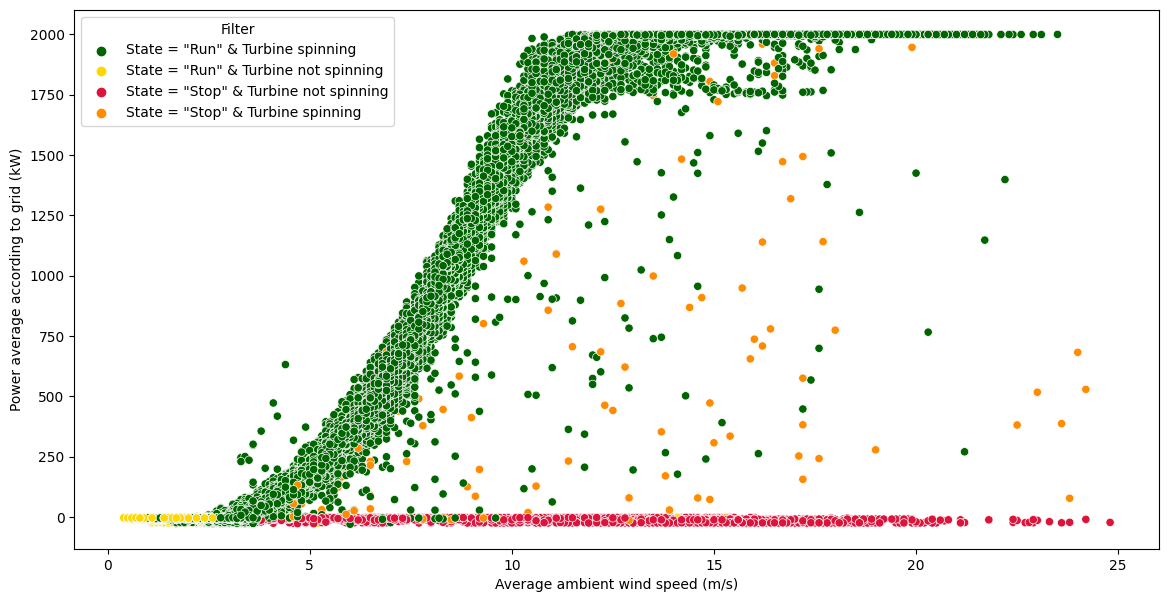
\includegraphics[scale=0.45]{Experiments/labels.png}
        \end{center}
        \caption{Turbine 01 power curve: Data points labeled based on different filters}
        \label{fig:labels}
      \end{figure}
    
      \subsection{Results}
      Here, we simply compared the models' performances by measuring their RMSE scores. Comparing the models' anomaly detection 
      and performance evaluation capabilities wasn't in the scope of this work, as we mainly focused on analyzing the generator-related condition 
      monitoring models. We did however reach these results while analyzing different strategies to utilize the SCADA logs in the 
      context of SCADA-based condition monitoring and decided they were worth documenting.\\

      Table \ref{tab:Experiment IV results} shows the measured RMSE scores of the three models. As shown, filtering the data improved
      the model's performance drastically. The filtering based on the turbine's state retrieved from the SCADA logs (\emph{Model-Run}) 
      yielded the best results in this setting. This shows that the generated labels provide valuable insights into the turbine's state 
      and can be used instead of a simple filter by the rotor's speed, especially if the latter isn't available as a SCADA signal for a given turbine.
      Figure \ref{fig:3pcs} also shows the better power curve fit both \emph{Model-Spin} and \emph{Model-Run} have compared to the \emph{Baseline} model 
      when applied to the testing dataset.

      \begin{table}[H]
        \centering
    \begin{tabular}{|c|c|c|c|}
    \hline
         \textbf{Metric} & \textbf{\emph{Baseline}} & \textbf{\emph{Model-Spin}} & \textbf{\emph{Model-Run}}\\
         \hline
         Training RMSE & 179.200 & 61.707 & 51.309\\
         \hline
         Testing RMSE & 139.972 & 59.988 & 50.251\\
    \hline
    \end{tabular}
    \caption{Experiment results: RMSEs measured and used to compare between the \emph{Baseline} model, \emph{Model-Spin} and \emph{Model-Run} when applied to Turbine 01}
        \label{tab:Experiment IV results}
    \end{table}

    \begin{figure}[H]
        \begin{center}
          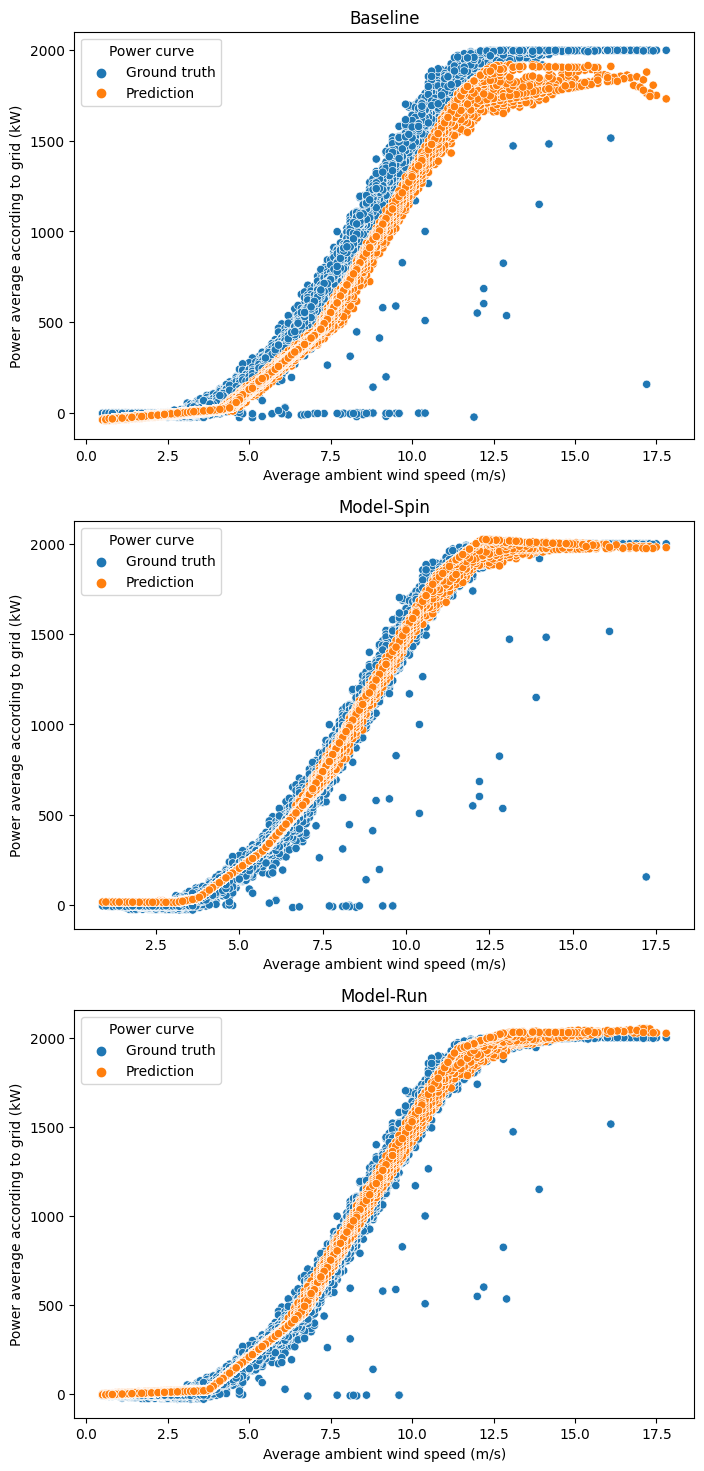
\includegraphics[scale=0.5]{Experiments/3pcs.png}
        \end{center}
        \caption{True versus predicted power curves of the \emph{Baseline} model, \emph{Model-Spin} and \emph{Model-Run}, respectively, 
        when applied to the testing dataset of Turbine 01}
        \label{fig:3pcs}
      \end{figure}
    

